% s6results.tex

\ac{S6} began on 7 July 2009 and ran until 20 October 2010. It overlapped two Virgo runs: \ac{VSR2}, which ran from 7 July 2009 to 11 January 2010, and \ac{VSR3}, which ran from 11 August 2010 to 20 October 2010. A number of improvements were made in both instrument hardware and \ac{CBC} analysis software between \ac{S5} and \ac{S6}. The software improvements have already been detailed in prior chapters: New \ac{SNR} was developed to replace effective \ac{SNR}, and Pipedown was implemented.

In this chapter we detail the \ac{S6} and VSR2/3 analysis. Section \ref{sec:hardware_improvements} describes some of the hardware improvements made to the detectors between \ac{S5} and \ac{S6}. In section \ref{sec:s6_epochs} we describe each of the four epochs the analysis was broken into. Section \ref{sec:dq_issues} details some of the major \ac{DQ} issues that arised during \ac{S6} and how they were dealt with, along with tuning decisions made. In this section we give an example of a veto developed from the loudest-slide studies that were implemented in the second half of \ac{S6}. Finally, in section \ref{sec:s6_results_and_big_dog} we give the results of the search, and we describe a blind injection that was made, and found, during \ac{S6}/VSR3. We do not present upper limits here as they are still being computed.

\section{Hardware Improvements}
\label{sec:hardware_improvements}

The two $4\,$km \ac{LIGO} interferometers, H1 and L1, were used for \ac{S6}.
The $2\,$km Hanford detector, H2, that is described in the last chapter was not
operational. Several hardware changes were made to the \ac{LIGO} detectors so
that prototypes of advanced LIGO technology could be installed and tested. This
included the installation of a more powerful, $35~\mathrm{W}$ laser, and the
implementation of a DC readout system that included a new Output Mode Cleaner
on an advanced LIGO seismic isolation table~\cite{Adhikari:2006}. In addition,
the hydraulic seismic isolation system was improved by fine-tuning its
feed-forward path. Known as HEPI feed-forward, this improvement was implemented
in January of 2010; it is described in more detail in section \ref{sec:s6b},
below.

Several hardware enhancements were also made to the Virgo detector in the
period between \ac{VSR1} and \ac{VSR2}. A more powerful laser was installed,
along with a thermal compensation system and scattered light was better
mitigated. During early 2010, monolithic suspension was installed, which
involved replacing Virgo's test masses with new mirrors hung from fused-silica
fibers. Following this upgrade Virgo began \ac{VSR3}. 

The average sensitivity of the detectors to binary coalescence signals in each epoch is shown
in Figures \ref{fig:s6a_insprange} -- \ref{fig:s6d_insprange}. These figures show the distance at
which an optimally oriented and located binary would produce a \ac{SNR}
of $8$ in a given detector. The figures show how the detectors were improved over the course of the run, until the eventually surpassed the best \ac{S5} ranges. 

\section{S6 Epochs}

\ac{S6} and VSR2/3 were broken into four epochs: \emph{S6A}, which ran from 7 July 2009 to 1 September 2009; \emph{S6B}, 24 September 2009 to 11 January 2010; \emph{S6C}, 6 February 2010 to 25 June 2010; \emph{S6D}, 26 June 2010 to 20 October 2010. Figure \ref{fig:s6_insprange_v_time} shows a plot of the \ac{BNS} inspiral range (with each component mass $= 1.4\,\Msun$) across all of \ac{S6} and the span of each epochs. The start and end times of the epochs were based on a combination of instrumental and analysis factors. S6A ended at a pre-planned commissioning break to try to improve the detectors after learning lessons from the first two months of running. S6B ran from the end of the commissioning break until the end of \ac{VSR2}. At this point, Virgo was taken off line for eight months in order to install the monolithic suspension. S6C therefore consisted only of double coincident time between Hanford and Livingston. Another commissioning break was taken at the end of S6B, hence the gap between the end of S6B and the start of S6C. S6D was to begin when Virgo came back online in August of 2010. However, during S6C we noticed that templates with total masses $> 25\,\Msun$ often rang off due to glitches. Thus we decided to lower the low-mass template bank from $2 \leq \mtotal/\Msun \leq 35$ to $2 \leq \mtotal/\Msun \leq 25$. We wanted to do this as soon as possible, and so the somewhat arbitrary date of 26 June 2010 was chosen as the break between S6C and S6D. Aside from Virgo eventually coming back online, there were no major instrumental adjustments between S6C and D. There were, however, new vetoes implemented for S6D based on \ac{CBC} results in S6C. These new vetoes, as well as more details about the decision to lower the template bank, are discussed in section \ref{sec:dq_issues}. In the next few sections we give more details about each of the epochs.

\begin{landscape}
\begin{figure}[p]
\begin{center}
\label{fig:s6_insprange_v_time}
\includegraphics[width=9in]{figures/s6-hzrange_v_time.png}
\end{center}
\caption{The inspiral range for a $1.4/1.4\,\Msun$ \ac{BNS} system at \ac{SNR} $8$ in each \ac{IFO} across \ac{S6}. The range is computed by \texttt{lalapps\_tmpltbank} using equation \ref{eqn:DtoRho}. Each dot represents the range in a $2048\,$s--long analysis chunk.}
\end{figure}
\end{landscape}

\clearpage

\begin{figure}[p]
\begin{center}
\label{fig:s6a_insprange}
\includegraphics[width=6in]{figures/s6a_insprange.pdf}
\end{center}
\caption{Average inspiral range of S6A. Ranges were computed by \texttt{lalapps\_tmpltbank} using equation \ref{eqn:DtoRho} with $\rho=8$, then averaged over all analysis chunks in the epoch. S6 ranges are in color; best S5 ranges are in gray. Although H2 was not used in \ac{S6}, it is shown for comparison to V1.}
\end{figure}

\begin{figure}[p]
\begin{center}
\label{fig:s6b_insprange}
\includegraphics[width=6in]{figures/s6b_insprange.pdf}
\end{center}
\caption{Average inspiral range of S6B. Ranges were computed using the same method as in Figure \ref{fig:s6a_insprange}.}
\end{figure}

\begin{figure}[p]
\begin{center}
\label{fig:s6c_insprange}
\includegraphics[width=6in]{figures/s6c_insprange.pdf}
\end{center}
\caption{Average inspiral range of S6C. V1 is not shown as it was down for commissioning during this period. Ranges were computed using the same method as in Figure \ref{fig:s6a_insprange}.}
\end{figure}

\begin{figure}[p]
\begin{center}
\label{fig:s6d_insprange}
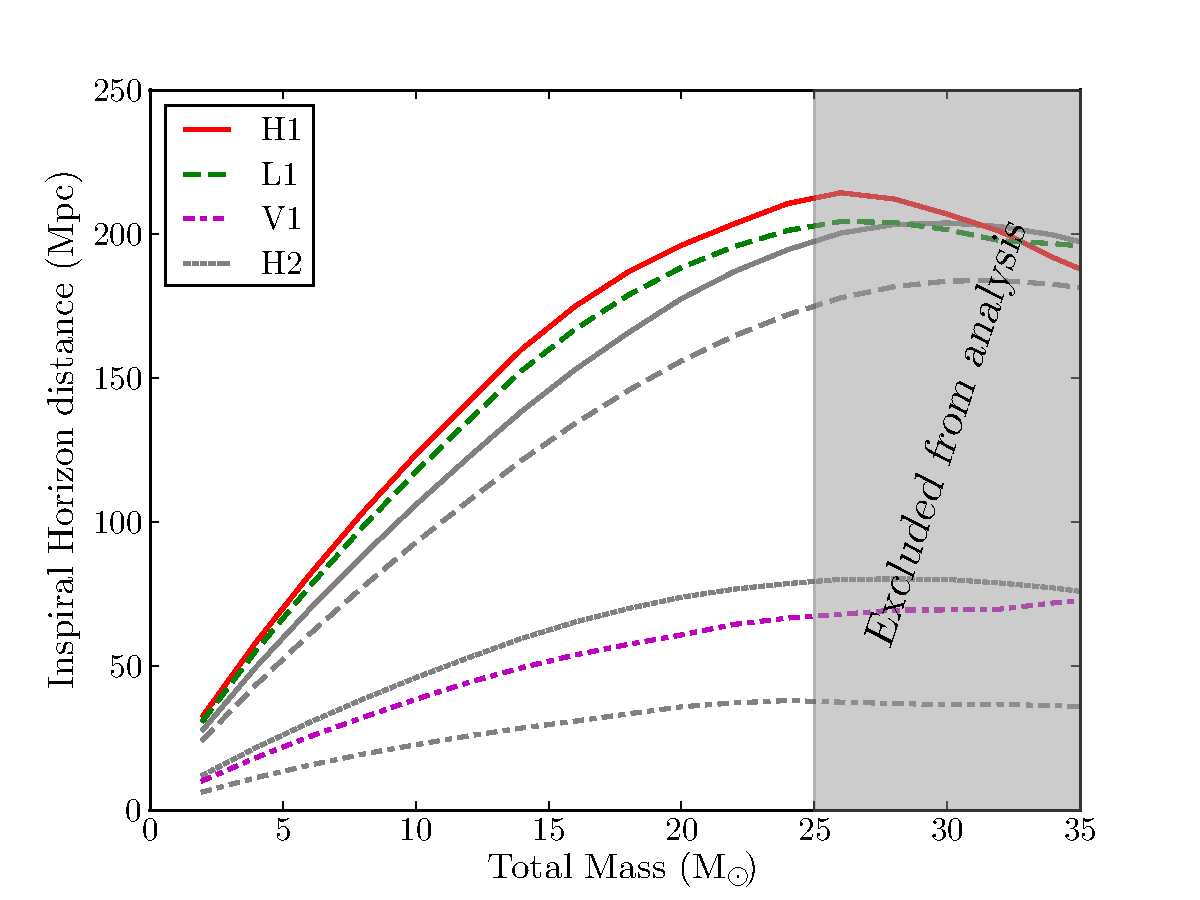
\includegraphics[width=6in]{figures/s6d_insprange_alt.pdf}
\end{center}
\caption{Average inspiral range of S6D. Shaded region indicates the mass range that was excluded in the low mass search for this period. Ranges were computed using the same method as in Figure \ref{fig:s6a_insprange}.}
\end{figure}

\subsection{S6A}
\label{sec:s6a}

Being the start of a new Science run, the \ac{LIGO} detectors had lower sensitivity and more glitches in S6A than in later epochs. This can be seen in Figure \ref{fig:s6_insprange_v_time}. In fact, the S6A \ac{LIGO} ranges were somewhat lower than they had been during their peak sensitivity in \ac{S5}. Figure \ref{fig:s6a_insprange} shows the average inspiral range versus binary total mass during S6A as compared to best ranges of \ac{S5}. We can see that Virgo, however, showed much improvement over VSR1, and had better sensitivity than H2 at its best in \ac{S5}.

In the \ac{S5}-LV search false alarm rates were based on a likelihood statistic that took into account the relative sensitivites of various interferometer combinations. The sensitivies were used to apply a weighting factor to each coincidence type so that more senstive \ac{IFO} combinations were promoted, allowing false alarm rates to be computed once across all combinations (as opposed to using equal-weighted bins to compute combined \acp{FAR} from uncombined). This was implemented for two main reasons: first, with both H2 and V1 active, four interferometers had to be analyzed, which led to an unwiedly number of coincidence types and instrument times to consider. Second, Virgo's sensitivity was much lower than the \ac{LIGO} detectors in VSR1, and, due to high amounts of low-frequency noise, its low-frequency cutoff had to be set to $60\,$Hz. Thus its template bank was truncated to have a maximum chirp mass of $\sim2.6\,\Msun$ \cite{ref:s5lvc}. The probability that various coincidence types detected a \ac{GW} was therefore far from equal, and so some sort of re-weighting needed to be applied. As can be seen in Figure \ref{fig:s6a_insprange}, however, the range of V1 was substantially better in \ac{VSR2} --- better than H2 --- and we were able to lower its low-frequency cutoff so that it could cover the same mass range as \ac{LIGO}. Essentially, V1 had taken the place of H2. Further, since V1 was not co-located with the other detectors, we could slide all the instruments against each other, which allowed us to analyze all instrument times. (Recall from the last chapter that H1 and H2 could not be slid against each other because they were co-located, and so H1H2 time could not be analyzed.) For these reasons, compounded with the fact that the \ac{S5}-LV likelihood method was still being developed when S6A started, we decided to analyze \ac{S6} in the same manner as in the \ac{S5} 12-18 month search, using combined \ac{FAR} as our ranking statistic, and with all the coincidence types being given equal weight. We also used many of the same tuning parameters as the \ac{S5} 12-18 month search: the \ac{SNR} cut, $\chi^2$ and $r^2$ veto thresholds, chirp-mass bins, and size of the ethinca parameter all remained the same.

There were a few minor adjustements, however. As mentioned in Chapter \ref{ch:pipeline_principles}, we switched to using 3.5 restricted \ac{pN} templates, although the template bank metric was still calculated using the 2\ac{pN} approximation. New \ac{SNR} was implemented as our ranking statistic for computing uncombined \acp{FAR} after it was noticed --- in the 12-18 month search and the S6A high-mass search --- that effective \ac{SNR} tended to over-weight triggers with statistically low $\chi^2$ values. Pipedown replaced older, more cumbersome, scripts to do post-\ac{HIPE} processing. As discussed in Chapter \ref{ch:ihope_pipeline}, we decided to do coincidence clustering within each chirp-mass bin as opposed to across all bins, as done in the 12-18 month search. We also switched algorithms for computing combined \acp{FAR} from the method discussed in section \ref{sec:alternate_cfar_method} of Chapter \ref{ch:far} to using slide triggers' uncombined \acp{FAR}, discussed in section \ref{sec:multiple_templates}. This change had little effect on the analysis, as they are equivalent. In the 12-18 month search, \ihope was run on month-long blocks of data as opposed to the year-long block used in the \ac{S5} first-year search. We continued this trend of decreasing the analysis periods in \ac{S6}: in S6A we decided to try to run \ihope on week-long blocks, with a different analyst being in charge of each period. Thus, S6A was (initially) broken into 8 week-long runs.

Initially we also planned to use trigscan clustering in \verb|lalapps_inspiral| to cluster triggers across templates. However, we were surprised to find that trigger rates were much higher than in \ac{S5}. They were so high that trigscan clustering was unable to keep the rate low-enough for many Inspiral jobs to finish (recall from Chapter \ref{ch:ihope_pipeline} that a disadvantage of trigscan is that it cannot garauntee a maximum trigger rate). Many jobs took several days to finish, or would simply run out of memory. As a result, only two weeks out of the eight were able to finish. Figure \ref{fig:avg_rate_per_tmplt} shows a comparison of the average trigger rate-per-template between one of the weeks that finished (``S6aWk3") and one of the months from the \ac{S5} LV analysis (``lvMonth8") at each stage of the pipeline. The rate was clearly higher for both H1 and L1 at all stages in the pipeline. In particular, the rate at second inspiral (2 on the x-axis) was not much lower than first inspiral (0 on the x-axis), implying that $\chi^2$ was being calculated for a large number of triggers. As this comparison had to use one of the weeks that finished, the other weeks that did not finish most likely had an even higher rate as compared to \ac{S5}.

To mitigate the high rates we decided to switch from trigscan to time-window clustering. What size window to use was an open question and so we used the two weeks that completed to investigate various clustering windows. We aimed to find the smallest window that allowed the search to continue, and that resulted in the most efficient recovery of vetoes. Three windows were considered: $10\,$ms, $30\,$ms, and $100\,$ms. The $10\,$ms window was found to be too short: the trigger rates were still too high for many runs to complete. This left the $30\,$ms and $100\,$ms windows. Figure \ref{fig:roc_cluster_windows} shows an ROC plot using $30\,$ms and $100\,$ms clustering. Note that in this plot we also considered raising the low-frequency cutoff to $65\,$Hz. As can be seen, the $30\,$ms window with the standard $40\,$Hz low-frequency cutoff provided the best results. We therefore decided to use the $30\,$ms clustering for all of \ac{S6}. Why trigscan clustering did not work as well is an open question. It may have simply been due to the high trigger rate. Another possibility is the switch from 2\ac{pN} to 3.5\ac{pN} templates somehow affected its ability to properly cluster. We plan to re-address this before advanced \ac{LIGO}.

\begin{figure}[p]
\center
\subfigure[H1]{\includegraphics[width=3in]{figures/s6_clusterwin_investigation/H1_average_rate_per_tmplt_comparisons.png}}
\subfigure[L1]{\includegraphics[width=3in]{figures/s6_clusterwin_investigation/L1_average_rate_per_tmplt_comparisons.png}}
\subfigure[V1]{\includegraphics[width=3in]{figures/s6_clusterwin_investigation/V1_average_rate_per_tmplt_comparisons.png}}
\label{fig:avg_rate_per_tmplt}
\caption{The average trigger rate per template in week 3 of S6A as compared to one month from the \ac{S5} LV analysis. Each point represents a different stage in the pipeline: $0 \rightarrow$ \texttt{INSPIRAL\_FIRST}, $1 \rightarrow$ \texttt{THINCA\_FIRST}, $2 \rightarrow$ \texttt{INSPIRAL\_SECOND}, and $3 \rightarrow$ \texttt{THINCA\_SECOND}. Stages $4$--$7$ represent the higher-category vetoes being applied at \texttt{THINCA\_SECOND}; there is an extra stage in S6A because hardware injections were removed by an extra veto-category (between steps $5$ and $6$), whereas in the LV search hardware injections were removed as apart of the CAT2 vetoes (at step $4$).}
\end{figure}

\begin{figure}[p]
\label{fig:roc_cluster_windows}
\center
\includegraphics[width=5in]{figures/s6_clusterwin_investigation/s6week3cat4_ROC.png}
\caption{ROC plot from week 3 of S6A using various clustering windows and low-frequency cutoffs.}
\end{figure}

%Show Andy's found-missed plots? They are here: https://www.lsc-group.phys.uwm.edu/ligovirgo/cbcnote/S6Plan/091123101532AnalysisS6a_lowmass_reruns#Clustering_and_missed_injections

\subsection{S6B}
\label{sec:s6b}

S6B began after the commissioning break in September of 2009. While the sensitivity in H1 improved slightly, the sensitivity in L1 was lower than in S6A. Further, L1 struggled to stay in lock for most of the period, and so the duty cycle was much lower. This can be seen in \ref{fig:s6_insprange_v_time}: note that L1 is off for large periods of time. The cause for the trouble was largely due to weather. As stated above, S6B ran from September to January. Fall brings a number of storms to the Gulf of Mexico, resulting in heightened \emph{microseismic} ($0.1$--$0.35$ Hz) noise. This made it difficult to keep the interferometer in lock.

To mitigate the seismic problem at Livingston HEPI feed-forward was developed during S6B. HEPI stands for Hydraluic External Pre-Isolation. Many of the interferometer's optics are sit on tables housed in vacuum chambers. These chambers are situated on hydraulic actuators, which are used to dampen out seismic noise. In the feed-forward process, the output from seismometers on the floor were fed into the actuators to cancel out the seismic motion, much in the same way noise-cancelling headphones work \cite{ref:Lundgren_comm}. The digital filters used in the feed-forward were implemented and tuned across S6B. This led to L1 becoming more stable, allowing for longer lock stretches. The effect can be seen in Figure \ref{fig:s6_insprange_v_time}: a few days prior to 16 December L1 suddenly starts staying in lock for longer periods of time. The increased stability eventually also allowed the laser power to be turned up to $14\,$W\footnote{The laser power was set to $14\,$W at both H1 and L1 during the evening and on weekends --- when there was little seismic noise from human activity --- throughout S6C and D. During working hours, the laser was typical set to $10\,$W.} which in turn led to better range. Thus, although S6B largely had poor data, it resulted in better range later on.

Due to the poor sensitivity of the \ac{LIGO} detectors and L1's low duty cycle, we decided to analyze S6B in three chunks. The first lasted from the start of S6B until 11 November 2009, at which point the detectors were re-calibrated. The second and third chunks ran from 11 November to 11 December, and 11 December to 11 January, respectively.

\subsection{S6C}
\label{sec:s6c}

After V1 went offline in January of 2010, another commissioning break was taken to try to better improve the \ac{LIGO} detectors. Thus the S6C analysis began a couple of weeks after the end of S6B, on 6 February. As can be seen in Figures \ref{fig:s6_insprange_v_time} and \ref{fig:s6c_insprange}, the commissioning throughout S6A and B paid dividends during S6C and D: it was during these periods that the \ac{LIGO} detectors reached their peak sensitivity, surpassing that of \ac{S5}.

It was during S6C that Pipedown was completed,\footnote{Pipedown was used throughout S6A and B. However, for both of those periods, it could only produce tables of loudest zero-lag events and IFAR plots. An early form of the \ihope page and loudest events table was used for S6A. For S6B injection-finding, PrintMissed, and PrintSims tables were added. By S6C, loudest-slide tables were added along with PlotFM plots.} allowing for loudest-slide studies to be carried out. New data-quality tools were also finished, including daily \ihope and a DQ wiki page. This page, which was generated each week, brought together information from online analyses and veto tools, including daily \ihope, Omega online (a tool used by the Burst group of which Omega scans are apart), Hveto (for \emph{Hierarchical Veto}, this is a tool that hierarchically ranks various auxillarily channels as potential vetoes by the probability they caused triggers in the \ac{GW} channel \cite{ref:https://wiki.ligo.org/DetChar/HvetoDoc}), and UPV (for \emph{Used Percentage Veto}, this is a tool that looks for correlations between auxilarilly channels and the \ac{GW} channel; if a channel is strongly coupled for a set of triggers, it is used as a veto) \cite{ref:https://virgo.physics.carleton.edu/trac/UPV-trac/wiki}. We therefore implemented the following system to analyze the data:
\begin{itemize}
\item{Each week a different analyst would be assigned to do a \ac{DQ} study. This involved going through that week's DQ page and checking the e-log for potential issues that would affect the \ac{CBC} analysis. They would record their findings on the DQ page (being a wiki, it could be edited after it was generated) and present them on a weekly telecon devoted entirely to the S6 analysis.}
\item{A ``lead" analyst would run \ihope on two weeks' worth of data, with a ``second" providing support (e.g., if the lead could not make a call or was having trouble getting the analysis to complete, the second would provide help). We required that the lead analyst be one of the two people who did the DQ study for one of the weeks that the \ihope run covered. Thus the analyst would be intimately familiar with potential issues in his or her run.}
\item{The lead or second would generate a closed-box \ihope page after \ihope completed (typically a few days). We would look over the page on the S6 telecon, paying careful attention to loudest-slide events and nearby missed injections. We were particularily interested in slide events that had combined new \acp{SNR} greater than $11.3$ as this would prevent detecting a \ac{GW} with a \ac{SNR} $= 8$ in each detector. The DQ studies would be reviewed to see if any flags or events recorded in the e-logs could explain the loudest slides. If a flag was found that passed safety checks --- i.e., it did not veto injections --- it would be added to the veto-definer file as either a CAT2 or CAT3 veto. UPV vetoes were also added at this point at CAT3. The lead or second would then re-run second Thinca and Pipedown with these new vetoes (this typically took a few hours). The new closed-box page would be checked again to make sure no new vetoes could be derived and that there were no glaring problems. An open-box page would then be generated and presented on the full \ac{CBC} telecon to see if there were any \ac{GW} candidates.}
\item{This process would be repeated on successive weeks, with each new analysis using the updated veto-definer file from the previous two weeks. The analysis was thereby fine-tuned as S6C continued.}
\end{itemize}

This method of using loudest slide triggers resulted in a number of vetoes being generated specifically for the low-mass \ac{CBC} search. Many of these vetoes were one-time use flags that were based on a specific event that occurred at one of the detectors, such as a computer glitching on a paritcular day. However, the study did result in some long-term vetoes being implemented. Section \ref{sec:seismic_veto} gives an example of one of these vetoes. Routinely opening boxes also allowed us to decrease the latency between when data was taken and when results were obtained. By the end of S6C and throughout S6D we were opening boxes approximately two weeks after the data had been taken. 

The decision to decrease the low-mass template bank to $\mtotal \leq 25\,\Msun$ was made at the end of S6C based on results from obtained during the epoch. The decision was influenced by two points: first, we found that the templates in the $25$--$35\,\Msun$ range were often rung off by glitches. Nearly half of the top 10 loudest events came from this part of the bank in each of the two week periods, despite it covering less than a third of the total mass space. The loudest slide events in the medium and high chirp-mass bins were also largely dominated by this mass range. The other factor leading to the decision was that the high-mass \ac{CBC} search, which covers $25 \leq \mtotal/\Msun \leq 100$, overlapped the low-mass search in this region. This overlap was unneeded since the template placing algorithm in \texttt{lalapps\_tmpltbank} would adequately cover the $\mtotal = 25\,\Msun$ line within each search. We therefore had two questions to answer: first, what search did better in the $25 -- 35\,\Msun$ region, the low-mass or the high-mass? Second, if the high-mass search better and we reduced the low-mass template bank, what would the effect on the low-mass search be?

To answer the first question, we ran the low-mass search and high-mass pipeline on the same 3 weeks of data (weeks 11-14 of S6C) then compared how well they recovered injections in the overlap region. Figure \ref{fig:mass_investigation-plotfm_lowmass} shows the found/missed plot as a function of total mass in the overlap region for the low-mass search, and Figure \ref{fig:mass_investigation-plotfm_highmass} shows the same for the high-mass search. The high-mass search appears to do better: more injections are recovered at farther distances, and a few injections that were missed in the low-mass search are now found. That the high-mass search does better in the region is further supported by Figure \ref{fig:mass_investigation-plotroc}, which shows the ROC plot for injections in the overlap region.

The high-mass search clearly worked better in the overlap region, suggesting we should lower the low-mass bank. To see the effect a smaller bank might have on the low-mass search, a test run with the lower-bank was run over the first two weeks of S6C and compared to the original run, which had the full bank. Figure \ref{fig:smaller_bank_investigation-lowmass} shows the found/missed plot as a function of chirp-mass for the two runs (spinning injections are excluded in these plots). There are a few subtle differences. Several injections on the edge of the range are found with lower \acp{FAR} with the lower-bank. This is expected since the volume of parameter-space we are searching is smaller, effectively giving a smaller trials factor. Perhaps most notable is that a nearby injection that was missed with the full bank (the red-cross with a chirp mass of $\sim1.9\,\Msun$ and decisive distance of $\sim40\Mpc$) is found with 0 \ac{FAR} by the smaller template bank. This was investigated in more detail; it was found to have little to do with the choice of mass-range, however. For more details see section \ref{sec:mysterious_missed_injection}.

Only one injection jumps out as doing worse in the smaller-bank run: the one with $\mchirp \approx 3.8\Msun$ and decisive distance $\approx 18\Mpc$. In the full-bank run it was ``found", albeit with a large combined \ac{FAR} (signified by the orange dot in the full-bank plot). In the smaller-bank run it was missed (signified by the red cross). This injection never should have considered ``found" in the full-bank run, however: a followup investigation found that the injection was on top of a glitch. The glitch rang off a high-mass template; since \texttt{ligolw\_inspinjfind} only uses a time-window, it labelled it as ``found" even though the recovered parameters were not close to the injected. In the smalller-bank run, no templates were rung off by the glitch and so it was considered missed, as it should have been. Thus, this injections was another indication that the smaller bank was better suited for the low-mass search.
%Only two injections jump out as having worse \acp{FAR} with the smaller bank than with the full bank: an injection with $\mchirp \approx 3\Msun$ and decisive distance $\approx 30\Mpc$ (it is marked by a red dot in the smaller-bank plot) and an injection with $\mchirp \approx 4.5$ and decisive distance $\approx 20\Mpc$ (marked by a light-blue dot in the smaller-bank plot). Both of these were found with $0$ \ac{FAR} with the full bank. These two injections were both spinning injections, however. We know that we do not recover spinning injections very well Table \ref{tab:smaller_bank_investigation-spininj} shows more detail about these injections, including injected and recovered parameters. In both cases the triggers with the best combined new \ac{SNR} come from templates with higher masses than what was injected. This is due to the mis-match between spinning injections and the non-spinning bank. Most likely, because $\chi^2$ does not work as well with higher mass templates (as they have fewer cycles in band) injections ring off templates with higher masses than what was injected. 

Injections aside, another metric of interest was the effect of using the smaller bank on the loudest-slide events. Table \ref{tab:smalller_bank_investigation-loudest_slides} compares the three loudest slide triggers from the original run and from the new run. There was little difference in the low and medium chirp-mass bins, but the high mass bin shows clear improvement. The loudest high chirp-mass event with the full bank had a combined new \ac{SNR} of $11.78$ whereas with the smaller bank it is $9.64$. This means that an event in the high chirp-mass bin with \ac{SNR} $8$ in each \ac{IFO} (the \ac{SNR} on which we base projected detection capabilities) would now stick out above the background.

The lower-bank offered some clear advantages and little or no disadvantages. For this reason we decided that we should lower the bank for all subsequent runs. This decision was made as the analysis of the two weeks ending on 25 June 2009 was being completed. We therefore decided to stop S6C on that date, and have ``S6D" begin with the analysis starting on 26 June, with the smaller-bank in place. It was suggested that we go back and re-analyze all of the S6C weeks with the smaller bank. However, given the relatively minor differences in the found/missed plots, we decided against it. This decision was further bolstered by Figure \ref{fig:smaller_bank_investigation-roc}, which shows a ROC plot comparing the smaller bank and the full bank. The gain in volume was not considered large enough to warrant a re-analysis.

\begin{figure}[p]
\center
\subfigure[Results using the low-mass search.]{\label{fig:mass_investigation-plotfm_lowmass}\includegraphics[width=4.8in]{figures/lower_tmpltbank_investigation/lowmass_plotfm.png}}
\subfigure[Results using the high-mass search.]{\label{fig:mass_investigation-plotfm_highmass}\includegraphics[width=4.8in]{figures/lower_tmpltbank_investigation/highmass_plotfm.png}}
\label{fig:mass_investigation-plotfm}
\caption{Found/missed plots as a function of total mass in the overlap region ($25 \leq \mtotal/\Msun \leq 35$) between the low-mass and high-mass search. Plot generated by \texttt{ligolw\_cbc\_plotfm} by running on three weeks of S6C data.}
\end{figure}

\begin{figure}[p]
\center
\label{fig:mass_investigation-plotroc}
\includegraphics[width=5in]{figures/lower_tmpltbank_investigation/overlap_allinj_ROC.png}
\caption{ROC plot comparing the sensitive volume in the overlap region between the low-mass and high-mass \ac{CBC} searches. All injection used for this plot have $\mtotal/\Msun \in [25.0, 35.0]$.}
\end{figure}

\begin{figure}[p]
\center
\subfigure[Results using the full bank.]{\label{fig:smaller_bank_investigation-lowmass-full_bank}\includegraphics[width=4.8in]{figures/lower_tmpltbank_investigation/lowmass-plotfm_full_bank.png}}
\subfigure[Results using the smaller bank.]{\label{fig:smaller_bank_investigation-lowmass-small_bank}\includegraphics[width=4.8in]{figures/lower_tmpltbank_investigation/lowmass-plotfm_small_bank.png}}
\label{fig:smaller_bank_investigation-lowmass}
\caption{Found/missed plots as a function of total chirp mass. Both plots were generated by \texttt{ligolw\_cbc\_plotfm} using the first two weeks of S6C data. The top plot shows the results from using a template bank spanning $2 \leq \mtotal/\Msun \leq 35$ and the lower plot shows the resuts from using a $2 \leq \mtotal/\Msun \leq 25$ bank. Only non-spinning injections with total mass $\leq 25\,\Msun$ were used in each plot.}
\end{figure}

\begin{table}[p]
\label{tab:smalller_bank_investigation-loudest_slides}
\center
\begin{tabular}{| c | c | c | c | c |}
\hline
Chirp Mass Bin & Run & $\mchirp (\Msun)$ & $\mtotal (\Msun)$ & Combined New \ac{SNR} \\ 
\hline \hline
\multirow{2}{*}{Low} & Full Bank & 2.34 & 6.26 & 9.85 \\
                     & Reduced Bank & 2.68 & 10.37 & 9.81 \\
\hline
\multirow{2}{*}{Medium} & Full Bank & 5.36 & 18.88 & 10.63 \\
                        & Reduced Bank & 5.24 & 19.91 & 10.29 \\
\hline
\multirow{2}{*}{High}   & Full Bank & 12.87 & 29.61 & 11.78 \\
                        & Reduced Bank & 9.86 & 23.11 & 9.64 \\
\hline
\end{tabular}
\caption{Comparison of loudest slide events between low-mass \ac{CBC} runs, one using the full template bank ($2 \leq \mtotal/\Msun \leq 35$) and one using the reduced bank ($2 \leq \mtotal/\Msun \leq 25$). Results are taken from the first two weeks of S6C data. The low, medium, and high chirp-mass bins are defined as $\mchirp \in [0.0, 3.48), ~[3.48, 7.4),$ and $[7.4, \max(\mchirp)]$, respectively, where $\max(\mchirp)$ is the largest possible chirp mass with each bank.}
\end{table}

\begin{figure}[p]
\center
\label{fig:smaller_bank_investigation-roc}
\includegraphics[width=5in]{figures/lower_tmpltbank_investigation/lowmass-lininj_compare_ROC.png}
\caption{ROC plot comparing the sensitive volume between the smaller low-mass bank run and the original, full-bank, run. Only injections distributed uniformly in linear distance were used in this plot; log-distributed injections showed similar results.}
\end{figure}

\subsection{S6D}
\label{sec:s6d}

The method of analyzing data on two week periods that was pioneered during S6C was continued throughout S6D. There were a few differences between S6C and D: in addition to reducing the template bank, described above, we also implemented two new automated vetoes: SeisVeto and a ``SNR $> 250$" flag. These are discussed in more detail in sections \ref{sec:lvea_seismic} and \ref{sec:spike_glitch}, respectively. The other major difference from S6C was that VSR3 began during S6D.

Virgo came back online on 11 August 2009 to begin VSR3. As mentioned above, in the break between VSR2 and VSR3, monolithic suspension was installed in an effort to increase Virgo's range. Unfortunately, a mirror with an incorrect radius of curvature was installed in the process. As can be seen in Figure \ref{fig:s6_insprange_v_time}, this resulted in V1 having lower sensitivity than it did in VSR2. V1 was also more glitchy.

Given Virgo's reduced sensitivity, we were concerned about leaving H1V1 and L1V1 doubles in triple time in the data. As explained in Chapter \ref{ch:far}, if we use all the possible coincidence types in triple time, we have a trials factor of 12 (4 coincidence types $\times$ 3 chirp-mass bins). This means that the combined \ac{FAR} of all (loud) triggers (for which all categories are active) will be 12 times larger than the uncombined \ac{FAR}. In doing so we have treated all the coincidence types with equal weight. However, with V1's reduced sensitivity, it was far less probable that an H1V1 or L1V1 trigger was a gravitational wave than H1L1 or H1L1V1 triggers. That the combined \ac{FAR} H1L1 and H1L1V1 triggers would gain a factor of 12 due to the much weaker H1V1 and L1V1 triggers would clearly be an over-estimation of the \ac{FAR}. The simplest fix was to simply throw out H1V1 and L1V1 triggers in triple time. This would decrease the trials factor in triple time to 6. Before doing this, however, we investigated what the effect of throwing out these triggers would be. Namely, we wanted to know if any injections would be missed, and we wanted to weigh this against the decrease in \ac{FAR} for H1L1 and H1L1V1 triggers.

In order to perform the study, two weeks of S6D/VSR3 data were used (from 3 September to 18 September 2010). Both \verb|ligolw_cbc_cluster_coincs| and \verb|ligolw_cbc_cfar| have the ability to remove specific coincidence types from a database; thus we simply re-ran cFAR on the Pipedown database generated by the standard run to re-compute the combined \acp{FAR} with the H1V1 and L1V1 doubles in triple-time excluded. 

Figure \ref{fig:V1doubles-found_missed-orig} shows the H1L1V1-time found/missed plot for the original run (with V1 doubles included); Figure \ref{fig:V1doubles-found_missed-excluded} shows the same, but with the V1 doubles excluded. Some injections do appear to be missed when the V1 doubles are excluded. To get a better handle on how many, and whether or not they are really ``found" injections (as opposed to being a glitch within the injection-finding window), the plots in Figure \ref{fig:V1doubles-coinc_types} were created. The top plot shows found/missed injections in H1L1V1 time as a function of coincidence type in the original run (with V1 doubles in). There are clearly some H1V1 and L1V1 injections, some of which have 0 combined \ac{FAR}. To get a sense of how many of these injections are true injections, the bottom plot shows the accuracy of the recovered chirp mass: ``found" injections around 0.0 are most likely real injections. When more detailed information was printed off for some of these injections, it was found that their effective distance in V1 was lower than that in H1 or L1, meaning that, despite Virgo's poor over-all sensitivity, there were still small areas in the sky to which V1 was more sensitive due to the antenna patterns.

Still, the relative number of H1V1 and L1V1 injections found as compared to H1L1 or H1L1V1 is clearly small. To weigh the gain in detecting these extra few injections against the cost of doubling the trials factor, the ROC plot in  Figure \ref{fig:V1doubles-roc} was created. This plot compares relative sensitive volume from leaving H1V1 and L1V1 doubles in triple time (blue curve) to excluding them (green curve). While the two curves are roughly the same at high \acp{FAR}, removing the doubles provides more sensitive volume at lower \acp{FAR}, which is the region of most interest since we would never claim a detection at the higher \acp{FAR}. Note in particular that at lower \ac{FAR} the green curve has approximately half the \ac{FAR} as the blue curve at the same relative volume, as expected from the reduction in trials factor. Based on these results and the small number of injections that would be missed, we therefore decided to exclude H1V1 and L1V1 doubles in triple time from the analysis for S6D.\footnote{Note that we still kept all triggers in H1V1 and L1V1 time. Since these times are mutually exclusive from H1L1V1 and H1L1 time, leaving them in the analysis had no effect on the \acp{FAR} of H1L1 and H1L1V1 triggers. Thus we only stood to gain by considering these times.}

\begin{figure}[p]
\center
\subfigure[H1V1 and L1V1 doubles included.]{\label{fig:V1doubles-found_missed-orig}\includegraphics[width=4.8in]{figures/excluding_V1_doubles/plotfm_found_missed-orig.png}}
\subfigure[H1V1 and L1V1 doubles excluded.]{\label{fig:V1doubles-found_missed-excluded}\includegraphics[width=4.8in]{figures/excluding_V1_doubles/plotfm_found_missed-excluded.png}}
\label{fig:V1doubles-found_missed}
\caption{Found/missed plots as a function of chirp mass in H1L1V1 time. The top plot includes H1V1 and L1V1 double-coincident triggers, the bottom plot was created with H1V1 and L1V1 coincidences excluded. Both plots created by \texttt{ligolw\_cbc\_plotfm} using two weeks of S6D/VSR3 data.}
\end{figure}

\begin{figure}[p]
\center
\subfigure[Decisive distance v. coincidence type.]{\label{fig:V1doubles-coinc_types-dist}\includegraphics[width=4.8in]{figures/excluding_V1_doubles/plotfm-dist_v_coinc_type-orig.png}}
\subfigure[Recovered chirp mass accuracy v. coincidence type.]{\label{fig:V1doubles-coinc_types-mchirp}\includegraphics[width=4.8in]{figures/excluding_V1_doubles/plotfm-mchirp_recovery_v_coinc_type-orig.png}}
\label{fig:V1doubles-coinc_types}
\caption{Found injections as a function of the coincidence type that they were found with. Both plots were created by \texttt{ligolw\_cbc\_plotfm} using the same data as used in Figure \ref{fig:V1doubles-found_missed}.}
\end{figure}

\begin{figure}[p]
\center
\subfigure[Injections distributed uniformly in linear distance.]{\label{fig:V1doubles-roc-linear}\includegraphics[height=3.5in]{figures/excluding_V1_doubles/lininj_ROC.png}}
\subfigure[Injections distributed uniformly in log distance.]{\label{fig:V1doubles-roc-log}\includegraphics[height=3.5in]{figures/excluding_V1_doubles/loginj_ROC.png}}
\label{fig:V1doubles-roc}
\caption{ROC curves comparing relative sensitive distance in H1L1V1 time when H1V1 and L1V1 coincidences are included (blue curve) to when they are excluded (green curve). The top plot was created using injections distributed uniformly in linear distance; in the bottom injections were distrubted uniformly in log distance. Both plots created by \texttt{lalapps\_cbc\_plotroc} using the same data as used in Figure \ref{fig:V1doubles-found_missed}.}
\end{figure}


\section{DQ Issues}

In the above sections we have covered some of the data quality issues that arose during S6 that resulted in tuning changes. These were the elevated trigger rate, the switch to a smaller template bank, and the decision to drop H1V1 and L1V1 coincidences in triple time during S6D/VSR3. Here we detail a few \ac{DQ} issues that we found during \ac{S6} and how we dealt with them. The three \ac{DQ} topics listed here are by no means exhaustive. They are simply meant to highlight some results from detailed loudest-slide and other DQ studies.

\subsection{The H1 \texttt{LVEA\_SEISZ} Veto: An Example Veto using Loudest Slides}

As described in section \ref{sec:s6c}, during S6C and D we used the loudest-slide triggers from the low-mass \ac{CBC} search to identify potential new vetoes. Many of the resulting vetoes were one-use flags based on observations noted in the e-log of some event at the detector sites. However, the loudest-slide results did result in a few vetoes that were used extensively. Here we present an example of one of those flags, the H1 \verb|LVEA_SEISZ| veto.

When we looked at the initial closed-box \ihope page for weeks 13 and 14 of S6C (1 May -- 14 May 2009), we found that the loudest slide trigger in the high chirp-mass had a relatively large combined new \ac{SNR} of 13.4. The \ihope analysis of the next two weeks (15 May -- 28 May 2009) also revealed a relatively loud slide trigger, this time in the medium mass bin with a combined new \ac{SNR} of 11.9. Table \ref{tab:seisz-loud_slides-pre_veto} lists some details about these triggers. There were no entries in either the Hanford or Livingston e-logs to suggest a cause for these events. However, as can be seen in Figure \ref{fig:seisz-loud_slides}, the Omega scans of the H1 \ac{GW} channel showed similar signatures. When a full-Omega scan was run of every channel at Hanford, we found considerable seismic noise occuring in the \verb|LVEA_SEISZ| channel during both events. Figure \ref{fig:seisz-omega_scans} shows the scan from this channel during these events. The \verb|LVEA_SEISZ| channel monitors vertical ground motion in the \emph{LVEA}, which is the building that houses all of the interferometer's central optics, such as the beam splitter, intermediate test masses, and dark port, as well as the laser.\footnote{The x and y channels also picked up motion. We used the z channel as it was found to be the most efficient at targeting resulting glitches in the \ac{GW} channel.}

We therefore developed a flag that monitored the RMS value of the \verb|LVEA_SEISZ| channel in the $3$--$10\,$Hz band \cite{ref:https://wiki.ligo.org/DetChar/H1LVEASEISZS6Cflag}. When the channel exceeded 1000 counts (counts are an arbitrary unit used for \ac{LIGO} channels; they are a measure of the amplitude of the channel), the flag would go off. Efficiency studies found the flag to be good at targetting noise transients caused by the seismic noise, with little ``deadtime" (this is how much time the flag is on for). It was therefore added as a CAT3 veto. Table \ref{tab:seisz-loud_slides-post_veto} shows the loudest events in the high and low chirp-mass bin in weeks 13 and 14 and weeks 15 and 16, respectively, after the application of the veto. The noise has dropped substantially, and is now below a combined new \ac{SNR} of $11.3$.

Initially, we only intended to use the flag for weeks 13-16 of S6C. Studies on the later weeks found that the flag became even more efficient, however, and so the flag was entered into online monitors as \verb|H1:DMT-BRMS_SEISMIC_LVEA_Z_3_10_HZ_THRESH_1E3|; it was used as a veto until the end of S6C. As we had already opened boxes on weeks 1-12, we did not apply it to those weeks. Further studies showed it would not have been as effective during those weeks, anyhow. Why this is, and what the cause was for the increased seismic noise in later weeks of S6C, is unknown. It may have been due to dam run-off near the Hanford observatory \cite{ref:Lundgren_comm}.

In S6D the \verb|LVEA_SEISZ| veto was superceded by SeisVeto. SeisVeto improved on \verb|LVEA_SEISZ| by used multiple seismic channels. The output from these channels were loaded into the Hveto algorithm along with daily \ihope triggers to find the strongest correlated channels each day. This automation gave even better efficiency with very little deadtime \cite{ref:https://wiki.ligo.org/DetChar/SeisVeto}. For more details on SeisVeto, see \cite{ref:SeisVeto} (in preparation).

\begin{figure}[p]
\center
\subfigure[H1 \ac{GW} channel at 957127982.06 (the loudest-slide event in weeks 13 and 14).]{\includegraphics[width=5in]{figures/lvea_seisz-veto/957127982_07_H1-LSC-DARM_ERR_1_00_spectrogram_whitened.png}}
\subfigure[H1 at 958413266.29 (the loudest-slide event in weeks 15 and 16 of S6C).]{\includegraphics[width=5in]{figures/lvea_seisz-veto/958413266_290_H1_LSC-DARM_ERR_1_00_spectrogram_whitened.png}}
\label{fig:seisz-loud_slides}
\caption{Omega scans of the gravitational-wave channel (\texttt{DARM\_ERR}) during the loudest-slide events shown in Table \ref{tab:tab:seisz-loud_slides-pre_veto}.}
\end{figure}

\begin{figure}[p]
\center
\subfigure[H1 \texttt{LVEA\_SEISZ} at 957127982.06 (the loudest-slide event in weeks 13 and 14).]{\includegraphics[width=5in]{figures/lvea_seisz-veto/957127982_07_H0-PEM-LVEA_SEISZ_512_00_spectrogram_whitened.png}}
\subfigure[H1 \texttt{LVEA\_SEISZ} at 958413266.29 (the loudest-slide event in weeks 15 and 16 of S6C).]{\includegraphics[width=5in]{figures/lvea_seisz-veto/958413266_290_H0_PEM-LVEA_SEISZ_512_00_spectrogram_whitened.png}}
\label{fig:seisz-loud_slides}
\caption{Omega scans of the \texttt{LVEA\_SEISZ} channel during the loudest-slide events shown in Table \ref{tab:tab:seisz-loud_slides-pre_veto}.}
\end{figure}

\begin{table}[p]
\label{tab:seisz-loud_slides-pre_veto}
\center
\begin{small}
\begin{tabular}{| c | c | c | c | c | c | c |}
\hline
\parbox[c]{1.5cm}{Analysis Period}   &   \parbox[c]{1.8cm}{Chirp-mass Bin}   &   $\mchirp (\Msun)$   &   $\mtotal (\Msun)$   &   \parbox[c]{1.8cm}{Combined New \ac{SNR}}   &   \ac{IFO}   &   \parbox[c]{2.5cm}{Single-\ac{IFO} \\End Time \\(GPS seconds)} \\
\hline \hline
\multirow{2}{*}{1 -- 14 May}    &   \multirow{2}{*}{High}    &   \multirow{2}{*}{12.7}   &   \multirow{2}{*}{33.3}    &   \multirow{2}{*}{13.4}    &   H1  &   957127982.06 \\
    &   &   &   &   &   L1  &   957128122.02 \\
\hline
\multirow{2}{*}{15 -- 28 May}   &   \multirow{2}{*}{Medium} &   \multirow{2}{*}{4.0}    &   \multirow{2}{*}{18.8}  &   \multirow{2}{*}{11.9}   &   H1  &   958413266.29 \\
    &   &   &   &   &   L1  &   958413311.36 \\
\hline
\end{tabular}
\end{small}
\caption{The loudest-slide events in the high chirp-mass bin of weeks 13 and 14, and in the medium chirp-mass bin of weeks 15 and 16, respectively, of S6C prior to application of the \texttt{LVEA\_SEISZ} veto. (Being the loudest slide events in their respective bins, both of these events had 0 combined \ac{FAR}.) Both of these events were found to be caused by seismic noise at Hanford.}
\end{table}

\begin{table}[p]
\label{tab:tab:seisz-loud_slides-post_veto}
\center
\begin{tabular}{| c | c | c | c | c | c | c |}
\hline
\parbox[c]{1.5cm}{Analysis Period}   &   \parbox[c]{1.8cm}{Chirp-mass Bin}   &   $\mchirp (\Msun)$   &   $\mtotal (\Msun)$   &   \parbox[c]{1.8cm}{Combined New \ac{SNR}}   &   \ac{IFO}   &   \parbox[c]{2.5cm}{Single-\ac{IFO} \\End Time \\(GPS seconds)} \\
\hline \hline
\multirow{2}{*}{1 -- 14 May}    &   \multirow{2}{*}{High}    &   \multirow{2}{*}{9.1}   &   \multirow{2}{*}{25.4}   &   \multirow{2}{*}{10.1}    &   H1  &   957858489.74 \\
    &   &   &   &   &   L1  &   957858414.75 \\
\hline
\multirow{2}{*}{15 -- 28 May}   &   \multirow{2}{*}{Medium} &   \multirow{2}{*}{4.4}    &   \multirow{2}{*}{20.9}  &   \multirow{2}{*}{10.3}   &   H1  &   958306864.45 \\
    &   &   &   &   &   L1  &   958306784.5 \\
\hline
\end{tabular}
\caption{The loudest-slide events in the high chirp-mass bin in weeks 13 and 14, and in the medium chirp-mass bin in weeks 15 and 16, respectively, of S6C after the application of the \texttt{LVEA\_SEISZ} veto. (Being the loudest slide events in their respective bins, both of these events had 0 combined \ac{FAR}.)}
\end{table}

\subsection{The ``Spike" Glitch}

Loud, short, transients in L1 OMC. Show one of Andy's time-series plots. Also show an Omega scan, and \ac{CBC} triggers created by it. Unable to determine cause. We resolved to create an \ac{SNR} > 250 flag, and veto at CAT3. Duncan MacCleod and I were supposed to study the effect on nearby injections, but it appears to have never finished.

%\subsection{Mysterious Missed Injection}
%
%In the smaller bank investigation described in section \ref{sec:s6c}, we noted that a \ac{BNS} injection that was in range was missed in the run with full template bank, but was found with zero combined \ac{FAR} with the smaller bank. (It can be seen as the red cross with $\mchirp \approx 3\,\Msun$ and decisive distance $\approx 40\,\Mpc$ in Figure \ref{fig:smaller_bank_investigation-lowmass-full_bank}.) We investigated this injection in more detail to understand why.

\section{Results}

As described in section \ref{sec:s6_epochs}, we initially analyzed the data in several small analysis periods --- weekly runs in S6a; three month-long chunks in S6B; bi-weekly run in S6C and D --- and opened boxes on each of these analyses. We did this so we could obtain results quickly, and so we could pro-actively adapt the pipeline to \ac{DQ} issues, as detailed above. However, we did this with the knowledge that we would have to re-run the pipeline over these periods. Re-runs were required in order to take advantage of final calibration studies, as well as fix minor issues in published veto segments.\footnote{Upon review, a CAT1 veto-flag was found to stay on (and off) for slightly longer periods than it should have. The effect on the analysis is small, however, amounting to a change in livetime of less-than a day across all of S6. For the sake of rigor, however, we have fixed the flag for re-runs.} For speed and simplicity these re-runs are being done in larger $\sim6$-week long chunks. S6A is being analyzed with one run; S6B is divided into two chunks, one prior to 11 November, and the other from 11 November to 11 January. S6C and D are each being re-analyzed in three chunks. Aside from the grouping of analysis runs together, no other changes have been made to the runs. For example, although new vetoes were created throughout S6C and D, these have not been retro-actively applied to earlier periods.

As the changes between the original runs and the final re-runs are minor, we do not expect our result to change. That is:
\begin{center}
\textbf{No gravitational-wave candidates were detected.}
\end{center}
Currently, the most significant trigger is an H1L1 trigger in H1L1V1 time with a
combined FAR of \firstFAR. The second and third most significant triggers had
combined FARs of \secondFAR~and \thirdFAR, respectively. All of these triggers
are consistent with background: having analyzed
$\mathrm{\sim0.5~yr}$~of data, we would expect the loudest event to
have a FAR of \expectedLoudestFAR. Although no detection candidates have been found,
 we will perform detailed follow-ups on the loudest triggers in each epoch once the re-runs have completed. These followups are carried out to aid in future \ac{DQ} investigations.

As apart of the re-runs we are performing extra injection runs. This is so we can improve our statistics for placing upper-limits. Since these runs are still on-going, and since the final upper limits will need to be reviewed once they are produced, we do not present upper-limits here.

% Estimate the UL using volume and time?

\section{The Blind Injection}

% original first mention
As apart of the {\it blind injection challenge}, a hardware injection was
injected into the \ac{LIGO} and Virgo detectors on \dogDate~at
\injectedDogTime~without the search groups' knowledge. The purpose of this was
to test the groups' abilities to detect signals and to exercise the LIGO and
Virgo Collaborations' procedures in the event that a real gravitational-wave
candidate is detected. The {\it blind injection} was found by the \ac{CBC}
group with a FAR low enough to be considered a detection candidate. We treated
the event as if it were real: detailed studies were done to establish the
significance and parameters of the event, and to vet the detectors of any
possible environmental or instrumental causes. Only after all procedures were
reviewed and a paper draft written was the event unveiled as an injection.
Although the event was not real, we present methods used to calculate the
significance of the event here, as they will be useful for future analyses.

% current paper introduction
The blind injection occurred on \dogDate~and was identified by multiple
searches. It was initially observed by a low-latency search for unmodeled
transients.  This search identified the injection as a gravitatioinal-wave
candidate with high significance in both LIGO detectors, chirping upward in
frequency from 40 to 400\,Hz. Virgo was observing with lower sensitivity and
did not show a significant signal. Coherent analyses showed that the lack of a
significant event in Virgo was consistent with the signal seen by the two LIGO
detectors. The observed chirp waveform was consistent with gravitational waves
radiated in the final moments of a coalescing compact binary system. The
detectors were in normal operation at the time of detection and no evidence
that the signal was of instrumental or environmental origin was found. The
event had a false alarm rate of less than \dogFAR in the search
reported here. After the analysis of the event was finished it was revealed 
to be a blind injection and removed from the data. 

% current paper discussion

The \ac{CBC} pipeline determined that a gravitational-wave candidate occurred
on \dogDate~at \recoveredDogTime, with \dogSNR in
coincidence between the two LIGO detectors in the {\it medium mass bin} ($3.48
\le \mathcal{M}/\Msun < 7.40$).  Virgo was also operating at the time of the
event, but its sensitivity was a factor of four lower than the LIGO detectors;
the absence of a signal in Virgo above the single-detector SNR threshold of 5.5
was consistent with this fact.  In the LIGO detectors, the signal was louder
than all time-shifted H1L1 coincident events in the same mass bin throughout
\ac{S6}. However, with only 100 time shifts, we could only bound the FAR to $<
1/23$ years, even when folding in all data from the entire analysis. To obtain
a better estimate of the event's FAR we performed all possible multiples of
5-second time shifts on four calendar months of data around the event,
corresponding to an effective analysis time of $2.0\times 10^5$
years, and considered only events with values of $\rho_{c} \ge 11$.  We found
five events with a value of $\rho_c$ equal to or larger than the
candidate's, as shown in Figure~\ref{fig:far}.  These five events were all
coincidences between the candidate's signal in H1 and time-shifted transient
noise in L1.  When we excluded 8 seconds from around the event's time in the
background estimation, we found {\em no}\/ background events with $\rho_c$
greater than the candidate and we obtained a significantly different background
distribution, also shown in Figure~\ref{fig:far}. 

\begin{figure}[tp]
\includegraphics[width=\columnwidth]{../s6-bigdog/Images/rate_vs_newsnr.png}
\caption{ The cumulative rate of events with chirp mass $3.48 \le
\mathcal{M}/\Msun < 7.40$ coincident in the H1 and L1, seen in four
months of data around the 16 September candidate, as a function of the
threshold ranking statistic $\rho_c$.  The blue triangles show
coincident events.  Black dots show the background estimated from 100
time shifts and black crosses show the extended background estimation
from all possible 5-second shifts on this data.  The gray dots and
crosses show the corresponding background estimates when a few seconds
of data around the time of the candidate are excluded.  Gray shaded
contours show the $1 - 5\sigma$ (dark to light) consistency of
coincident events with the estimated background including the extended
background estimate, for the events and analysis time shown, including
the candidate time.  This event was late revealed to have been a blind
injection. }
\label{fig:far}
\end{figure}


Including the events at the time of the candidate in the background estimate,
the FAR of the event in the $3.48 \le \mathcal{M}/\Msun < 7.40$ mass bin,
coincident in the LIGO detectors, was estimated to be \dogTrialFAR.
Since this event occurred in H1L1V1 time during VSR3, only two coincidence
types were considered: H1L1 double-coincident events and H1L1V1
triple-coincident events.  This resulted in a trials factor of 6 (accounting
for the three mass bins and two coincidence types) and a combined FAR of
\dogFAR.  The probability of a false alarm with this combined FAR
value or lower, in this analysis, was \dogFAP.

\begin{figure*}[htb]
\begin{center}
% 'hot' colorscheme plots
\includegraphics[width=2.42in]{../s6-bigdog/Images/omegagram_h1h.png}
\includegraphics[width=2.09in]{../s6-bigdog/Images/omegagram_l1h.png}
\includegraphics[width=2.09in]{../s6-bigdog/Images/omegagram_v1h.png}
\caption{A time-frequency decomposition of the signal power associated with the
detection event observed in the \ac{LHO} (left), \ac{LLO} (middle), and Virgo
(right) detectors~\cite{ref:omegagrams}.  The zero of time in these plots is
the event time reported above.  The ``normalized tile energy'' is roughly
equivalent to SNR$^2$/2 in a time-frequency tile. For Gaussian noise in the
absence of signal, the normalized tile energy rarely exceeds 8.  The images
from the LIGO detectors both show a significant signal with frequency
increasing over time, characteristic of compact binary coalescence.
This event was later revealed to have been a blind injection.}
\label{fig:omegagrams}
\end{center}
\end{figure*}

\begin{figure}[t]
\includegraphics[width=\columnwidth]{../s6-bigdog/Images/lal_strain_16sample_average.pdf}
\caption{Detector strain amplitude spectrum around the time of the injection:
\ac{LHO} in red, \ac{LLO} in green and Virgo in magenta.  At these noise
levels, an optimally located and oriented (5,5)$\Msun$ binary would give a
matched-filter signal-to-noise ratio (SNR) of 8 at distances of 120, 130 and 30
Mpc in LHO, LLO and Virgo respectively.  The diagonal lines show the strength
of binary coalescence signals observed in the LHO (solid) and LLO (dashed)
detectors with SNRs of 15 and 10, respectively, as explained in the text.
\label{f:noise_curve}}
\end{figure}

Figure~\ref{fig:omegagrams} shows time-frequency plots of the detector data
around the time of the injection. A ``chirp'' waveform was clearly visible in
the H1 and L1 data. This signal was also audible in the whitened detector
strain data. The highest matched-filter SNR obtained in the search was $15$ at
$\mathcal{M} = 4.7\,\Msun$ in H1 and $10$ at $\mathcal{M} = 4.4\,\Msun$ in L1.
This difference in SNRs is consistent with typical differences in antenna
response factors for these differently-oriented detectors.  The quantity
$|2\tilde{s}(f)\sqrt{f}|$, where $\tilde{s}(f)$ is the Fourier transform of the
best-matched filter waveform, can be directly compared with the strain noise
amplitude spectral density in each detector; this is shown in
Figure~\ref{f:noise_curve} to illustrate the strength of the signal seen in the
two LIGO detectors.

We performed an extensive investigation to check for any
non-gravitational-wave causes for the observed event. The injection
passed all checks performed. We performed a thorough study of the
coupling of environmental noise to the gravitational-wave channel. None
of the environmental monitors recorded a transient during the time of
the injection.  The LIGO observatories were in quiet night-time
operation with near maximum astrophysical range; the Virgo detector
had quiet environmental conditions, except for elevated micro-seismic
levels. Most mechanisms that could cause coincident signals among widely
separated detectors were ruled out. It is very unlikely that such mechanisms could
cause a signal that monotonically increases in frequency and is visible
in the LIGO data --- as seen in time-frequency spectrograms shown in
Figure~\ref{fig:omegagrams} --- without leaving a clear signature in the
environmental monitors. There were no significant earthquakes at the
time, and seismic up-conversion through the Barkhausen effect, harmonic
up-conversion or bilinear coupling were all ruled out as potential
causes. Acoustic coupling was also ruled out. No extraordinary
electromagnetic transients were seen at the observatories at the time,
and the worldwide electromagnetic ``weather'' was calm, ruling out, e.g.,
very low-frequency radio, whistlers, chorus and riser
signals~\cite{Singh:2004}.  Observatory cosmic ray detectors showed no
unusual activity.

A loud transient occurred in L1 9 seconds before the coalescence time of the
signal. The transient belonged to a known family of sharp ($\sim$ 10ms) and
loud (SNR $\approx 200$-$80000$) glitches that appear 10-30 times per day in
the output optical sensing system of this detector. Since the candidate signal
swept through the sensitive band of the detector, from 40 Hz to coalescence,
in less than 4 seconds, it did not overlap the loud transient.  Studies,
including re-analysis of the data with the glitch removed, indicated that the
signal was not related to the earlier instrumental glitch.  No evidence was
found that the observed signal was associated with, or corrupted by, any
instrumental effect.


\subsection{Conclusions}

In the S6 paper I draw on the upper-limits in the conclusion. Can I show preliminary upper limits?

\section{Extra Stuff}

(Next chapter)

The other investigation was the LIGO South investigation of whether or not we can detect at SNR 8 with two detectors. The wiki for this is linked from the April 13, 2010 CBC minutes. It was done using S5 data, so it doesn't seem to belong in this chapter. S5 chapter? Or at all? I allude to it in Chapter 2 we showing plots of snr and newsnr.

